\subsection{Results and scope}
The validation route is double box: off, sunrise: learned at $\tau=0.001$, vacuum3: learned at $\tau=0.0001$. Other topologies use native equation choices. The forced learned filter uses $\tau=0.001$, while the distance filter retains seeds with $\delta\leq 4$. These choices remain fixed throughout the held-out tests.

All 280 complete workflows reproduce their native reference coefficients. The independent audit checks 91,240 coefficient pairs, including 1,931 distinct expression pairs, by exact rational simplification in $d$. The workflows contain 40 failed filtered attempts before successful fallback, and their times include these attempts. Native median complete times range from 0.785 to 5.880 seconds across the fourteen batches.

The forced learned filter has a complete-time ratio of 1.080, with descriptive interval $[0.976,1.220]$. Its equation-preparation ratio is 1.053, with descriptive interval $[0.904,1.224]$. The generated-equation ratio is 0.769, and the selected-equation ratio is 0.985. All ratios use the matched native control, so a value below one indicates a lower measured cost.

The distance filter has a complete-time ratio of 1.016, with descriptive interval $[0.994,1.040]$. Its equation-preparation ratio is 1.089, with descriptive interval $[1.035,1.144]$. The generated-equation ratio is 1.000, and the selected-equation ratio is 1.000. All ratios use the matched native control, so a value below one indicates a lower measured cost.

The automatic route has a complete-time ratio of 1.098, with descriptive interval $[0.981,1.259]$. Its equation-preparation ratio is 1.062, with descriptive interval $[0.896,1.261]$. The generated-equation ratio is 0.849, and the selected-equation ratio is 1.000. All ratios use the matched native control, so a value below one indicates a lower measured cost.

The automatic route does not lower the aggregate complete time in this test. Equation-count changes therefore do not establish an overall runtime gain.

\begin{figure}[htbp]
 \centering
 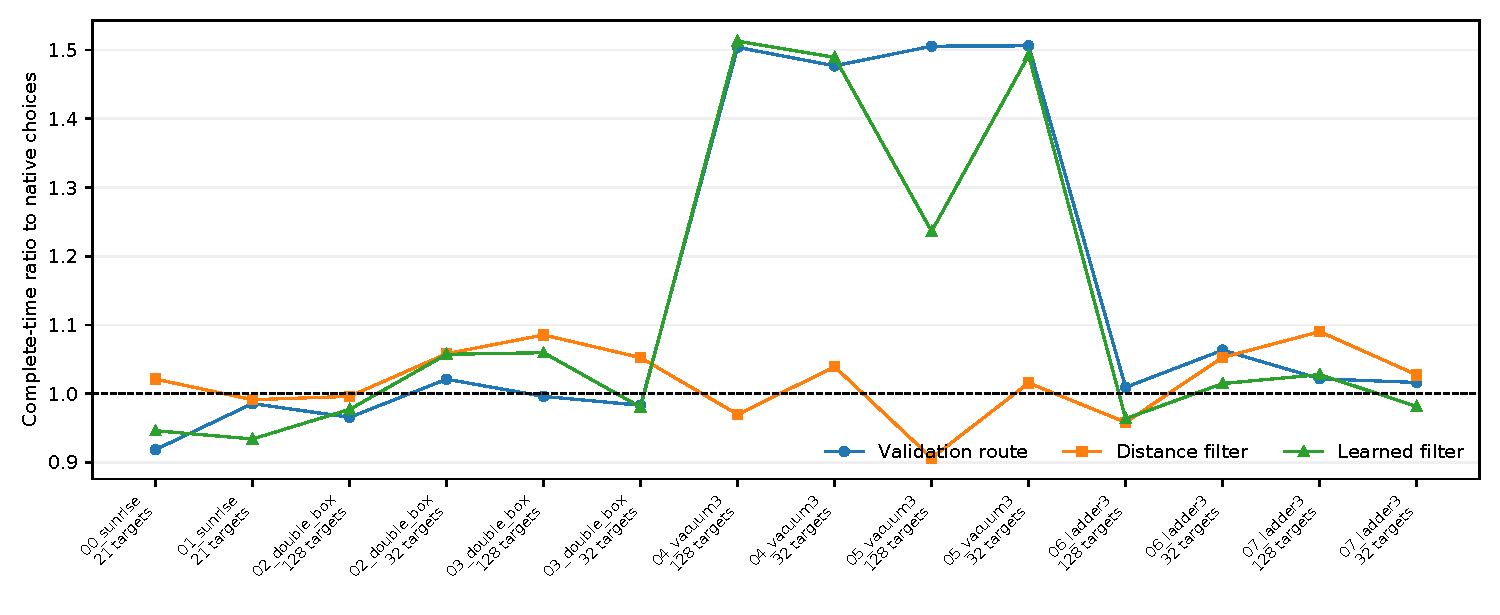
\includegraphics[width=\textwidth]{figures/equation_complete_times.pdf}
 \caption{Median complete-time ratios for the fourteen held-out batches.
 Each point uses five repetitions and includes checks and fallback.
 The dashed line is the native control.}
 \label{fig:equation-complete}
\end{figure}
\begin{figure}[htbp]
 \centering
 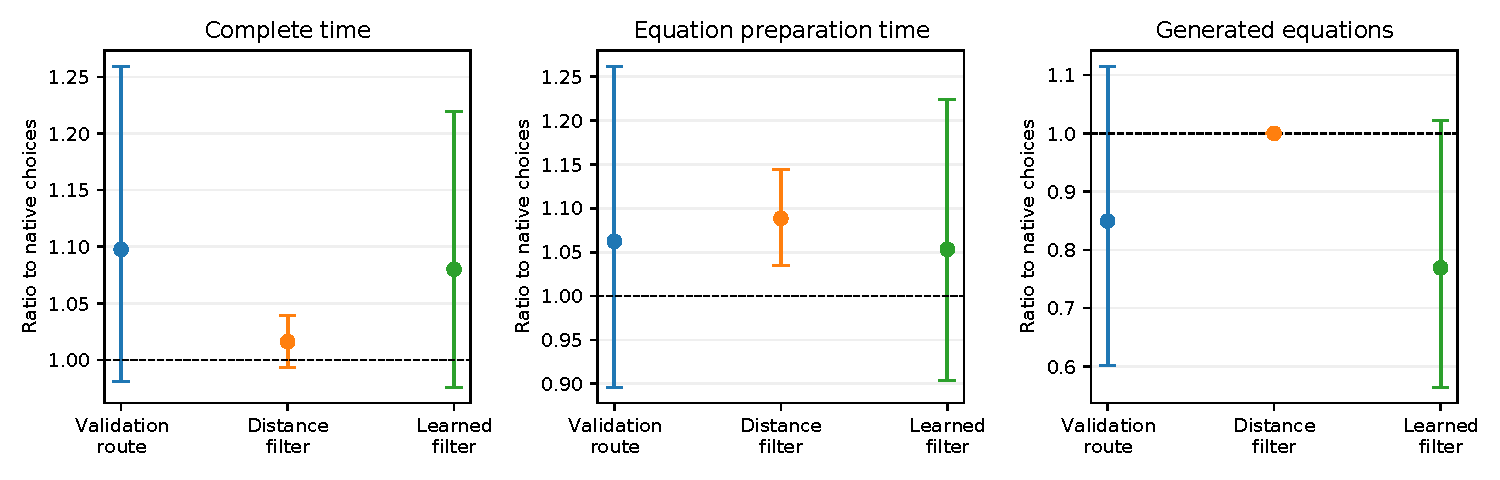
\includegraphics[width=\textwidth]{figures/equation_aggregate_costs.pdf}
 \caption{Profile-weighted geometric ratios of complete time, equation
 preparation time and generated-equation count. Bars show descriptive
 intervals from resampling the eight physical profiles.}
 \label{fig:equation-aggregate}
\end{figure}

After freezing the model, we also collect 77,246 held-out candidate labels, with 6,932 positive labels. At the forced learned threshold, precision is 11.33\% and recall is 95.63\%, with mean squared probability error 0.0621. These quantities measure agreement with the native support-membership proxy. Exact coefficient comparisons measure the validity of the resulting reductions.

\begin{figure}[htbp]
 \centering
 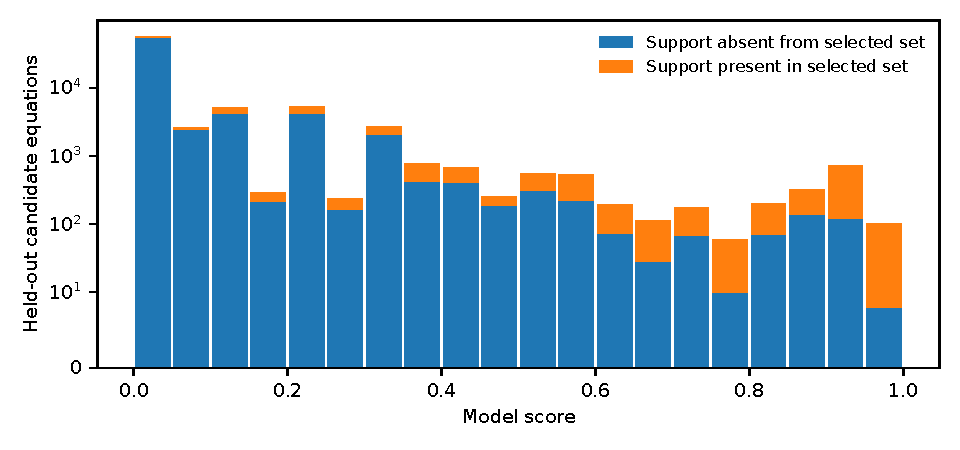
\includegraphics[width=.78\textwidth]{figures/equation_label_scores.pdf}
 \caption{Held-out model scores grouped by the native support-membership
 label. The vertical scale is linear near zero and logarithmic above ten
 equations. The labels describe selected supports rather than necessary
 equations.}
 \label{fig:equation-labels}
\end{figure}

A further 48 complete workflows test the equation route together with the existing row policy and with both existing policies on four profiles. Adding the equation route gives a complete-time ratio of 1.165 to the row-only configuration and 1.184 to the configuration with both earlier models. These comparisons use three repetitions and retain all fallback costs. All pass the reference checks. Eight application runs also pass exact coefficient comparisons after execution with reference coefficients withheld from the reducer.

The early full-feature implementation and subsequent feature-sharing implementations remain in the evidence collection, including their slower results. The final comparison uses the frozen implementation selected before held-out testing. Its performance depends on target size, topology and the cost of generating and reducing the retained equations. The experiment covers physical two- and three-loop reductions at fixed rational kinematics with symbolic $d$; it does not establish gains on arbitrary higher-loop or fully multiscale problems~\cite{KiraEquationSelectionData}.
\FloatBarrier

\subsection{The domain selected before testing}
Validation enables the equation model for the sunrise and three-loop vacuum topologies. This identifies four of the eight test profiles before any test timing is available. On these profiles, the automatic route has a complete-time ratio of 1.194, with descriptive interval $[0.951,1.498]$. Its equation-preparation ratio is 1.078, with descriptive interval $[0.765,1.519]$. The corresponding generated-equation ratio is 0.722.

For sunrise profiles, the automatic complete-time ratio is 0.951 and the preparation ratio is 0.765. For vacuum3 profiles, the automatic complete-time ratio is 1.498 and the preparation ratio is 1.519. For double box profiles, the automatic complete-time ratio is 0.991 and the preparation ratio is 0.988. For ladder3 profiles, the automatic complete-time ratio is 1.027 and the preparation ratio is 1.110. The double-box and ladder routes retain native equation choices, so differences between their automatic and native timings mainly reflect repeated-run variation and routing overhead. The all-profile comparison remains the primary result; these fixed-domain results state where the learned filter was active.

